\documentclass[10pt,a4paper]{article}

\usepackage[utf8]{inputenc}		% Configuro la codificación
\input{.command.tex}
% En el siguiente archivo se configuran las variables del trabajo práctico
%% \providecommand es similar a \newcommnad, salvo que el primero ante un 
%% conflicto en la compilación, es ignorado.

% Al comienzo de un TP se debe modificar los argumentos de los comandos


\providecommand{\myTitle}{TRABAJO PRÁCTICO}
\providecommand{\mySubtitle}{Ecualizador de audio digital}

\providecommand{\mySubject}{Procesamiento de señales (86.51)}
\providecommand{\myKeywords}{UBA, Ingeniería, PS1}

\providecommand{\myAuthorSurname}{Manso}
\providecommand{\myTimePeriod}{Año 2018 - 1\textsuperscript{er} Cuatrimestre}

% No es necesario modificar este %%%%%%%%%%%%%%
\providecommand{\myHeaderLogo}{header_fiuba}
%%%%%%%%%%%%%%%%%%%%%%%%%%%%%%%%%%%%%%%%%%%%%%%%

% Si se utilizan listings, definir el lenguaje aquí
\providecommand{\myLanguage}{matlab}

% Crear los integrantes del TP con el comando \PutMember donde
%%		1) Apellido, Nombre
%%		2) Número de Padrón
%%		3) E-Mail
\providecommand{\MembersOnCover}[0]
{		
		\PutMember{Lean Cole, Micaela} {96364} {leancolem@gmail.com}
		\PutMember{Manso, Juan} {96133} {juanmanso@gmail.com}
}

\providecommand{\myGroupNumber}{11}

\Pagebreaktrue		% Setea si hay un salto de página en la carátula
\Indextrue
\Siunitxtrue			% Si quiero utilizar el paquete, \siunixtrue. Si no \siunixfalse
\Todonotesfalse		% Habilita/Deshabilita las To-Do Notes y las funciones \unsure, \change, \info, \improvement y \thiswillnotshow.
\Listingstrue
\Keywordsfalse
\Putgroupfalse		% Habilita/Deshabilita el \myGroup en los headers
\Videofalse
				% Archivo con los comandos globales como Título y autores
%Preambulo para articulo científico de LaTeX

\usepackage[a4paper,left=3cm,right=3cm,bottom=3.5cm,top=3.5cm]{geometry} 	% Configuro la geometría del papel
%\usepackage{microtype}								% Mejora el "spacing" de las palabras
\usepackage[spanish]{babel} 							% Compatibilizo los signos del español
	\addto\captionsspanish{\renewcommand{\tablename}{Tabla}}		%% Redefino nombres preestablecidos por Babel
	\addto\captionsspanish{\renewcommand{\listtablename}{Índice de tablas}}	%% y así en vez de Cuadro dirá Tabla.
\usepackage{amsmath, amsfonts, amssymb}						% Entornos matemáticos, fuentes y símbolos
\usepackage{graphicx}								% Necesario para insertar figuras
\usepackage{fancyhdr}								% Para manipular headers y footers
\usepackage[usenames,dvipsnames]{color}						% \color{color deseado} {lo que querés que tenga color}
\usepackage{subcaption}								% Permite captions del tipo 1a, 1b
\usepackage{multirow}								% Para tablas
\usepackage{float}

% Para video
\ifVideo
	\usepackage{media9}
	\addmediapath{./../reportes/}
\fi

%\usepackage{times}
%\usepackage{mathtools}
\usepackage{upgreek} % letras griegas sin cursiva
%\usepackage{cancel}
\usepackage{rotating}
\usepackage{tikz}
\usepackage{pgfplots}
%	\pgfplotsset{compat=1.12}
	\usetikzlibrary{plotmarks}% matlab2tikz
\usepackage{grffile}% matlab2tikz 
	\usetikzlibrary{calc,patterns,decorations.pathmorphing,decorations.markings}

\ifListings
	\usepackage{listings}

	\providecommand{\lstinputpath}[1]{\lstset{inputpath=#1}}

%	\input{.lst_default.tex}
	\input{.lst_matlab.tex}
%	\input{.lst_c.tex}
%	\input{.lst_c++.tex}
	
% 	\input{.lst_pseudocode.tex}


\fi

\ifSiunitx
\usepackage{siunitx}											% Unidades: \SI {cantidad} {\unidad} (necesita texlive-science)
	\sisetup{load-configurations = abbreviations}							% Habilita poner \cm en vez de \centi\metre
	\sisetup{output-decimal-marker = {,}}									% Cambia los puntos decimales por comas
	\sisetup{per-mode = fraction}											% Pone las unidades como fracción
	\sisetup{quotient-mode = fraction}										
\fi


\ifTodonotes
\usepackage{xargs}
\usepackage[colorinlistoftodos,prependcaption,textsize=tiny]{todonotes}


	\newcommandx{\Juan}[2][1=]{\todo[linecolor=red,backgroundcolor=red!25,bordercolor=red,#1]{#2}}
	\newcommandx{\Gonza}[2][1=]{\todo[linecolor=blue,backgroundcolor=blue!25,bordercolor=blue,#1]{#2}}
	\newcommandx{\Maxi}[2][1=]{\todo[linecolor=OliveGreen,backgroundcolor=OliveGreen!25,bordercolor=OliveGreen,#1]{#2}}
	\newcommandx{\improvement}[2][1=]{\todo[linecolor=Plum,backgroundcolor=Plum!25,bordercolor=Plum,#1]{#2}}
	\newcommandx{\thiswillnotshow}[2][1=]{\todo[disable,#1]{#2}}
\fi


\usepackage{booktabs}														% Permite hacer tablas sin separadores en el medio
\usepackage{placeins}														
		\let\Oldsection\section												%% Permite que los flotantes (como figuras) no aparescan
	\renewcommand{\section}{\FloatBarrier\Oldsection}						%% antes o después de su sección correspondiente.
		\let\Oldsubsection\subsection
	\renewcommand{\subsection}{\FloatBarrier\Oldsubsection}		
		\let\Oldsubsubsection\subsubsection
	\renewcommand{\subsubsection}{\FloatBarrier\Oldsubsubsection}
\usepackage{hyperref}														% Debe ser agregado al final del preambulo

\hypersetup
{    bookmarks=true,         % show bookmarks bar?
     unicode=false,          % non-Latin characters in Acrobat’s bookmarks
     pdftoolbar=true,        % show Acrobat’s toolbar?
     pdfmenubar=true,        % show Acrobat’s menu?
     pdffitwindow=false,     % window fit to page when opened
     pdftitle={\myTitle},    		 % title
     pdfauthor={\myAuthorSurname},   % author
	 pdfcreator={\myAuthorSurname},	 % creator = author
     pdfsubject={\mySubject},		 % subject of the document
     pdfkeywords={\myKeywords},
     colorlinks=true,        % false: boxed links; true: colored links
     linkcolor=black,        % color of internal links (change box color with linkbordercolor)
     citecolor=black,        % color of links to bibliography
     filecolor=magenta,      % color of file links
     urlcolor=cyan           % color of external links
}

%Configuro la pagina con los encabezaos y pies de paginas
\pagestyle{fancy}										% Para agregar encabezados y pie de paginas	
\lhead{\mySubject}										% Encabezado izquierdo
\rhead{\includegraphics[scale=0.15]{\myHeaderLogo}} 	% Encabezado derecho (logo de la FIUBA)	
\ifPutgroup
\chead{\texttt{Grupo Nº\myGroupNumber} \\ \textit{\footnotesize{\myTimePeriod}}}
\fi				

%% Este archivo contiene las funciones auxiliares para escribir en LaTeX
%% Dichas funciones resuelven la sintaxis de generar figuras, por ejemplo,
%% dejando el código más compacto y facilitando la corrección del mismo.



% Comando para graficar eps. 1er arg, escala. 2do, ruta. 3ro, caption. 4to, label.
\providecommand{\HgraficarEPS}[4]{
			\begin{figure}[h!]
				\centering
					\scalebox{#1}{\input{#2}}
					\caption{#3}
					\label{#4}
			\end{figure}

}

\providecommand{\HgraficarPNG}[4]{
			\begin{figure}[h!]
				\centering
					\includegraphics[scale=#1]{#2}
					\caption{#3}
					\label{#4}
			\end{figure}

}


% Comando para graficar eps en el lugar previsto.
\providecommand{\graficarEPS}[4]{
			\begin{figure}[h]
				\centering
					\scalebox{#1}{\input{#2}}
					\caption{#3}
					\label{#4}
			\end{figure}

}

\providecommand{\graficarPNG}[4]{
			\begin{figure}[h]
				\centering
					\includegraphics[scale=#1]{#2}
					\caption{#3}
					\label{#4}
			\end{figure}

}

		% Se proveen un conjunto de funciones extras

% Defino el path de los includegraphics
\graphicspath{{./Figuras/}}		% Directorio que contiene los graficos

% Defino el path para los input de .tex y de .eps
\makeatletter
\def\input@path{{./Figuras/}{./Secciones/}{./Cover_page/}}
\makeatother

% Defino el path del listings
\ifListings
%% Cambiar el nombre de la carpeta si se utilizan Listings
	\lstinputpath{{../Octave/}}
\fi



\begin{document}
		% Carátula (formal o simple,_formal o _simple respectivamente) con Resumen
		% incluido e Índice (si es necesario configurar en config.tex) del informe
		\begin{titlepage}
	
		\thispagestyle{empty}

		\begin{center}
			
\includegraphics[scale=0.3]{fiuba}\\
			\large{\textsc{Universidad de Buenos Aires}}\\
			\large{\textsc{Facultad De Ingeniería}}\\
			\small{\myTimePeriod}
		\end{center}

		\vfill

		\begin{center}
			\Large{\underline{\textsc{\mySubject}}}
		\end{center}

		\vfill

		\begin{tabbing}
			\hspace{2cm}\=\+\myTitle\\
				TEMA: \mySubtitle\\
				FECHA: \today\\
			\\
				\MembersHeader
				\MembersOnCover	
		\end{tabbing}

		\begin{abstract}
			% Ejemplo de Resumen
%% MANTENER EL NOMBRE %%
	El siguiente trabajo práctico tiene como objetivo el diseño de filtros para utilizar como ecualizador de audio digital.



		\end{abstract}

	\ifKeywords
		\begin{center}
			\emph{Palabras Clave: \myKeywords}
		\end{center}
	\fi	

		\vfill
	
\end{titlepage}

\ifPagebreak
	\thispagestyle{empty}
	\ifIndex
		\tableofcontents
%		\listoffigures
%		\listoftables
	\fi

	\pagebreak
\fi


	\setcounter{page}{1}

	\section{Especificaciones}\label{sec:specs}
		El ecualizador de audio digital a diseñar debe cumplir los siguientes requerimientos:

\begin{itemize}
	\item \SI{2}{\dB} de desviación máxima sobre la línea ideal (respuesta plana);
	\item la compensación debe abarcar el rango de frecuencias $\SI{20}{\Hz}$- $\SI{16}{\kilo\Hz}$ (un poco menor al rango audible).
	\item se deben utilizar la menor cantidad de recursos, es decir, el menor orden posible del filtro ecualizador.
\end{itemize}

		
	\section{Parte I: Ecualización mediante filtros de fase lineal}\label{sec:partei}
		
\subsection{Método de ventanas}

Se desea implementar el ecualizador mediante un filtro que no agregue distorsión de fase. Para ello se utilizan los filtros \emph{FIR FLG}. En esta sección se diseña y caracteriza un filtro mediante el método de ventanas.

% \lstinputlisting[firstline=30, lastline=76]{tp.m}

	\subsubsection{Ítem a: amplitud del ecualizador}

% Definir A_{EQ}(w) con sus correspondientes bandas, amplitudes, tolerancias (ripple) adecuadas para cumplir los requerimientos, frecuencias de corte, paso y supresión.

%La frecuencia de muestreo es de $f_s = \SI{44.1}{\kilo\Hz}$. 
	Primero se realiza la transformada rápida de Fourier o \textit{fft} de 1024 puntos de la señal que entrega el sistema electroacústico. Esta señal es la que se tiene como dato en el archivo \textit{SEA.mat}.\\

Para obtener las bandas de interés, se calculan los extremos locales de esta curva, teniendo en cuenta que se puede acotar el rango de frecuencias de interés de la señal desde los $\SI{20}{\Hz}$ hasta los $\SI{16}{\kilo\Hz}$\footnote{El rango audible de frecuencias para el humano adulto es $\SI{20}{\Hz}$ - $\SI{20}{\kilo\Hz}$. Para los fines de este trabajo práctico, se ha decidido acotar un poco más las frecuencias agudas al valor mencionado.}, ya que se trata de una señal de audio.\\

	\graficarEPS{0.6}{graf_P11a_sistema_EA}{Módulo de la respuesta en frecuencia del sistema electroacústico original.}{fig:P11a_sistema_EA}
	
	Como primera aproximación, se obtienen los extremos utilizando la función \textit{findpeaks}, que devuelve tanto la ubicación de cada máximo como el valor del mismo. Para hallar los mínimos, se aplica la misma función pero al módulo de la respuesta inversa del sistema. Luego, los límites de las bandas para el filtro son los valores promedio entre cada máximo y mínimo consecutivo. En la Figura \ref{fig:P11a_sistema_EA} se muestra el resultado de dicho proceso.\\

% La curva azul representa el módulo de la respuesta en frecuencia del sistema electroacústico; en verde se marcan los límites de las frecuencias de interés mencionadas, escaladas según el valor de la frecuencia de muestreo; los puntos rojos son los extremos locales obtenidos; las bandas de interés están delimitadas por las líneas punteadas amarillas.\\

%	En la Figura \ref{fig:P11a_sistema_EQ} se muestra la respuesta del filtro multibanda y la del sistema original:
%
%	\begin{figure} [H]
%		\centering
%		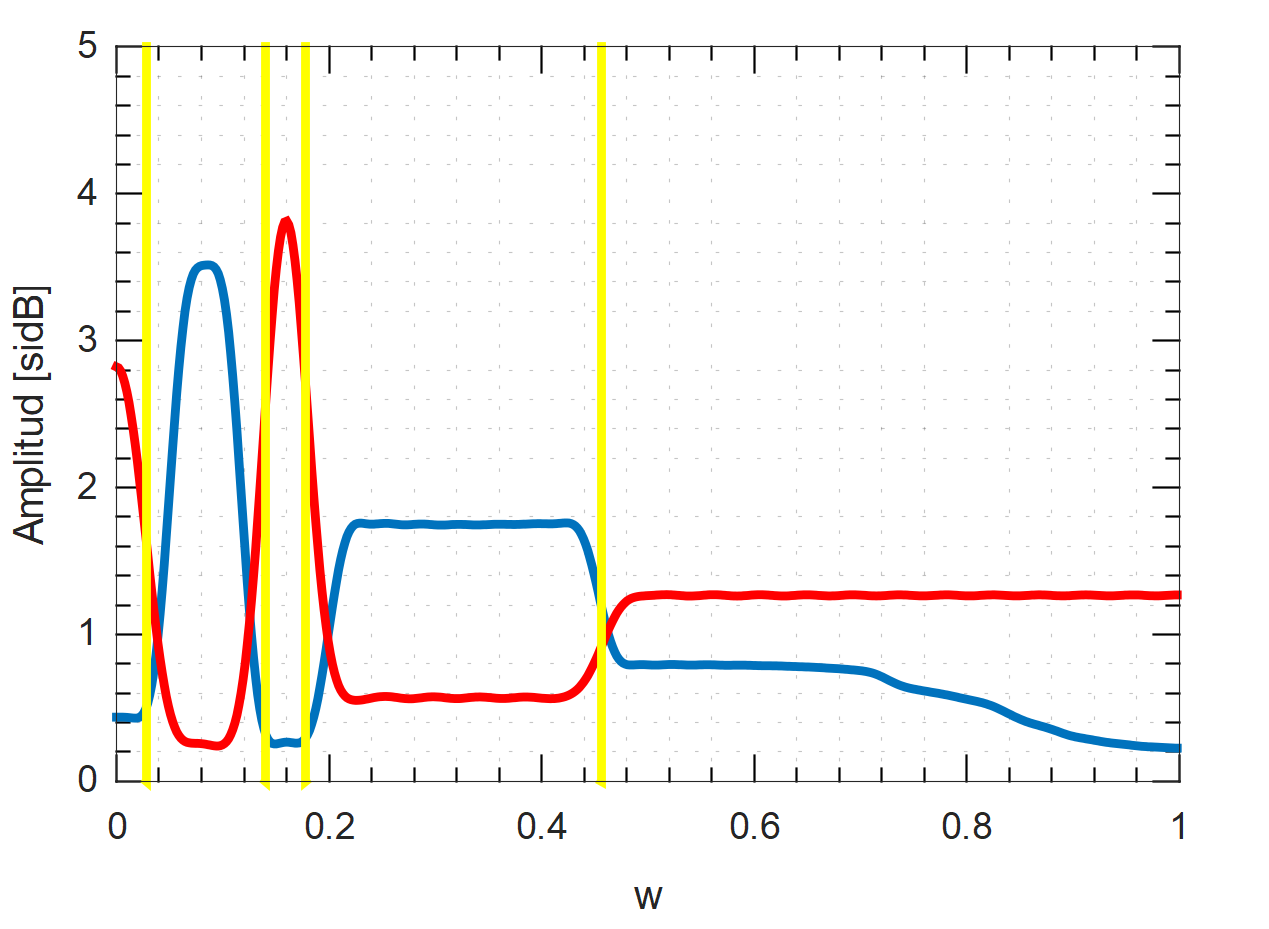
\includegraphics[width=0.9\textwidth]{P11a_sistema_EQ.png}
%		\caption{\label{fig:P11a_sistema_EQ}Módulo de la respuesta en frecuencia del filtro ecualizador y del sistema electroacústico original.}
%	\end{figure}
%
%La curva azul representa el módulo de la respuesta en frecuencia del sistema electroacústico; la curva roja representa la del filtro multibanda diseñado; las bandas de interés están delimitadas por las líneas amarillas.\\
%
%Se obtienen los siguientes valores para los parámetros de cada banda:
	
	Según hipótesis, la tolerancia es de \SI{2}{\dB} que equivale a $\delta_0 = 0.01$ de magnitud. Sin embargo, para la utilización de ventanas se debe hacer un escalamiento de las tolerancias correspondientes a cada banda. Para normalizar las tolerancias $\delta$ del sistema electroacústico, se realiza el cociente $\delta_i = \delta_0 / a_i$ donde $a_i$ es la ganancia de la i-ésima banda.\\

	En la Tabla \ref{tab:specs} se exponen las caracterísitcas de la función amplitud $A_{EQ}(w)$ del filtro a implementar. Por inspección se obtiene que $\max \{\delta_i\} = \delta_3 \approx 0.04$. Este valor implica que no hay restricción de qué ventana utilizar, dado que la que tiene el $\delta$ más pequeño es la \emph{rectwin} con $\delta_{rectwin} = 0.09$ y es mayor que $\delta_3$.

	Por último se decidió no definir las bandas de paso y supresión de cada caso. En el caso que fuese necesario obtener estos valores, se obtendrán a partir del valor de $w_c$ y la suma (o resta) de un $\Delta w = \num{0.025}\cdot\pi$.

	\begin{table}[h!]
		\centering
		\begin{tabular}{*{6}{c}}
			\toprule
			Parámetro	&	Banda 1 & Banda 2 & Banda 3 & Banda 4 & Banda 5\\
			\midrule
			Frecuencias límites ($\frac{w_c}{\pi}$)	& $0$ - $0.050$	& $0.050$ - $0.120$	& $0.120$ - $0.203$	& $0.203$ - $0.456$	& $0.456$ - $0.726$\\
			Ganancia		& $2.327$	& $0.284$	& $3.933$	& $0.569$	& $1.267$\\
			Tolerancia ($\delta_i$)	& $0.023$	& $0.003$	& $0.039$	& $0.006$	& $0.013$\\
			\bottomrule
		\end{tabular}
		\caption{Especificaciones para el filtro a implementar.}
		\label{tab:specs}
	\end{table}


	\subsubsection{Ítem b: filtro multibanda}

	Previo a la construcción del filtro ecualizador, se diseña la función \texttt{multibanda(a,w,M,win)} que se encarga de generar el filtro deseado a partir de suma y/o restas de filtros pasa-bajos. Para corroborar el correcto funcionamiento de dicha función, se propone generar un filtro cuya respuesta en frecuencia coincida con la respuesta del sistema. De este modo se puede también verificar que los datos especificados en la Tabla \ref{tab:specs} sean correctos (utilizando como alturas la inversa de las ganancias expuestas en dicha Tabla).\\

	Como la longitud del lóbulo principal más pequeño de la respuesta del sistema electroacústico (segunda banda) se supuso como $\Delta w = 0.1\pi$, para una ventana rectangular se obtiene que $M_{rectwin}=41$. En la Figura \ref{fig:P11b_seguidor_rectwin} se presenta el filtro que sigue la respuesta del sistema utilizando la ventana rectangular. 
	
	Dado que el \emph{ripple} generado por la ventana es mayor a la tolerancia aceptable, se opta por seguir a la señal por medio de una ventana de \emph{Hamming}. Se puede ver en la Figura \ref{fig:P11b_seguidor_hamming} que al aumentar el orden, el filtro consigue replicar el comportamiento de la respuesta del sistema. Las diferencias pueden deberse al efecto de los lóbulos secundarios que disminuyen los valores pico de la segunda y tercer banda. Con un ajuste de las amplitudes podría conseguirse una curva más cercana.\\
	
	\HgraficarEPS{0.6}{graf_P11b_seguidor_rectwin}{Seguimiento de la respuesta del sistema EA por medio de \texttt{multibanda()} utilizando ventana rectangular.}{fig:P11b_seguidor_rectwin}
	
	\HgraficarEPS{0.6}{graf_P11b_seguidor_hamming}{Seguimiento de la respuesta del sistema EA por medio de \texttt{multibanda()} utilizando ventana de \emph{Hamming}.}{fig:P11b_seguidor_hamming}

	\pagebreak
	A partir del análisis expuesto en el párrafo anterior, y el ajuste de los parámetros, se obtiene el filtro ecualizador $H_{EQ}(w)$ utilizando $M=90$ y ventaneo de \emph{Hamming}. Se decidió por el filtro de tipo I (orden par; simétrico), para que no atenúe las frecuencias en $0$ ni en $\pi$. 
	De todas formas, si se hubiese implementado un filtro tipo II, al no poder escuchar tan bajas frecuencias (por el cero en 0), no sería un inconveniente.
	En la Figura \ref{fig:P11c_rta_frecuencia_eq} se ilustra el filtro ecualizador en conjunto con la respuesta del sistema. Al final de esta sección se provee una fracción del código utilizado para generar los gráficos expuestos con los respectivos parámetros.	

	\graficarEPS{0.6}{graf_P11c_rta_frecuencia_eq}{Módulo de la respuesta en frecuencia del filtro ecualizador.}{fig:P11c_rta_frecuencia_eq}

	\begin{lstlisting}
aux=[H(LOC2(1)) H(LOC(1)) H(LOC2(2)) H(LOC(2)) H(LOC2(end))];
% Copia de HSEA
%%%% RECTWIN %%%%
%	M = 41;
%	wc = [0.050 0.120 0.193 0.456];
%	a = aux;
%	tipo_ventana = @rectwin;
%
%%%% HAMMING %%%%
%	M = 90;
%	wc = [0.050 0.120 0.193 0.456];
%	a = aux;
%	tipo_ventana = @hamming;

%% Filtro ecualizador
	M = 90;
	wc = [0.028 0.140 0.178 0.456];
	a = [3.00 0.260 04.83 0.569 1.266];
	tipo_ventana = @hamming;

[heq, M] = multibanda(a,wc,M,tipo_ventana);
	\end{lstlisting}

	\subsubsection{Ítem c: respuesta en frecuencia y retardo de fase}
	
	Una vez implementado el filtro multibanda deseado, ilustrado en la Figura \ref{fig:P11c_rta_frecuencia_eq}, se calcula el producto de la respuesta del sistema con el filtro ecualizador. El resultado se ve en la Figura \ref{fig:P11c_rta_frecuencia_tot}. Se puede verificar que el filtro cumple los requerimientos iniciales de tolerancia y de ancho de banda. \\
	
	\graficarEPS{0.56}{graf_P11c_rta_frecuencia_tot}{Transferencia total del sistema tras la ecualización, graficado en decibeles.}{fig:P11c_rta_frecuencia_tot}

	Como se puede comprobar, se cumple con el requerimiento estipulado de la desviación máxima de \SI{2}{\dB}.

	También se grafica el retardo de fase del ecualizador, del sistema electroacústico y del sistema total, como en la Figura \ref{fig:P11c_retardo_fase}. Se puede observar que el retardo de fase que introduce el filtro, al ser de fase lineal, es constante igual a la mitad del orden como es de esperar. En consecuencia, sólo genera una traslación temporal evitando cualquier tipo de distorsión de fase.
	
	\HgraficarEPS{0.56}{graf_P11c_retardo_fase}{Retardo de fase del sistema EA, el ecualizador y el sistema total.}{fig:P11c_retardo_fase}
	
	Por tratarse de un filtro de fase lineal, todo el contenido de fase está en el término 
	{\color{red}{No entiendo esta oración y lo que quiere decir con la ecuación.... :S}}
	
	\begin{equation*}
			H_{EA}(z) = \prod^n_{k=1} \frac{1-c_k z^{-1}}{1} 
			\label{eq:prod_hea}
	\end{equation*}


%%%%%%%%%%%%%%%%%%%%%%%%%%%%%%%%%%%%%%%%%%%%%%%%%%%%%%%%%%%%%%%%%%%%%%%%%%%%%%%%%%%%%%%%%%%%%%%%%%%%%%%%%%%%%%%%%%%%%%%%%%%%%%%%%%%%%%%%%%%%%%%%%%

\subsection{Método de filtros óptimos}

En esta sección se diseña el filtro ecualizador mediante el método de filtros óptimos. Se analizan los mismos parámetros que con el método de ventanas para poder compararlos, tanto objetivamente como subjetivamente al probarlos con distintas señales de ejemplo. \\
{\color{red}{Tal vez hay que sacar lo de las señales de ejemplo...}}

% En proceso, en un rato lo pongo aca

	\subsubsection{Ítem a: amplitud del ecualizador}

	\graficarEPS{0.6}{graf_P12a_amplitud_eq}{Amplitud del filtro ecualizador.}{fig:P12a_amplitud_eq}
	
%	\begin{figure} [H]
%		\centering
%		\includegraphics[width=0.9\textwidth]{P12a_amplitud_eq.png}
%		\caption{\label{fig:P12a_amplitud_eq}Amplitud del filtro ecualizador.}
%	\end{figure}
	
	Puede verse que tiene mayor ripple que la amplitud del ecualizador con el método de ventanas.
	% Me falta


	\subsubsection{Ítem b: respuesta en frecuencia y retardo de fase}

	Al igual que en la sección anterior, se computa el módulo de la respuesta en frecuencia del ecualizador resultante así como la del sistema total.\\
	
	\graficarEPS{0.56}{graf_P12b_rta_frecuencia_tot}{Transferencia total del sistema tras la ecualización, graficado en decibeles.}{fig:P12b_rta_frecuencia_tot}
	
	Como se puede observar en la Figura \ref{fig:P12b_rta_frecuencia_tot}, hay una banda para la cual el requerimiento estipulado inicialmente no se cumple, ya que la amplitud se extiende en dos picos que superan lo que se considera de banda plana (un pico negativo que llega hasta los \SI{-3}{\dB} y uno positivo hasta los \SI{5}{\dB}, aproximadamente). Estos sobrepicos que superan la tolerancia requerida se deben a la falta de control sobre la banda de transición que se tiene al diseñar mediante cuadrados mínimos. Se podría solucionar suavizando las discontinuidades de $A_d(w)$.\\


	También se grafica el retardo de fase del ecualizador, del sistema electroacústico y del sistema total, como en la Figura \ref{fig:P12b_retardo_fase}:

	\HgraficarEPS{0.60}{graf_P12b_retardo_fase}{Retardo de fase del sistema EA, el ecualizador y el sistema total.}{fig:P12b_retardo_fase}
	
%	\begin{figure} [H]
%		\centering
%		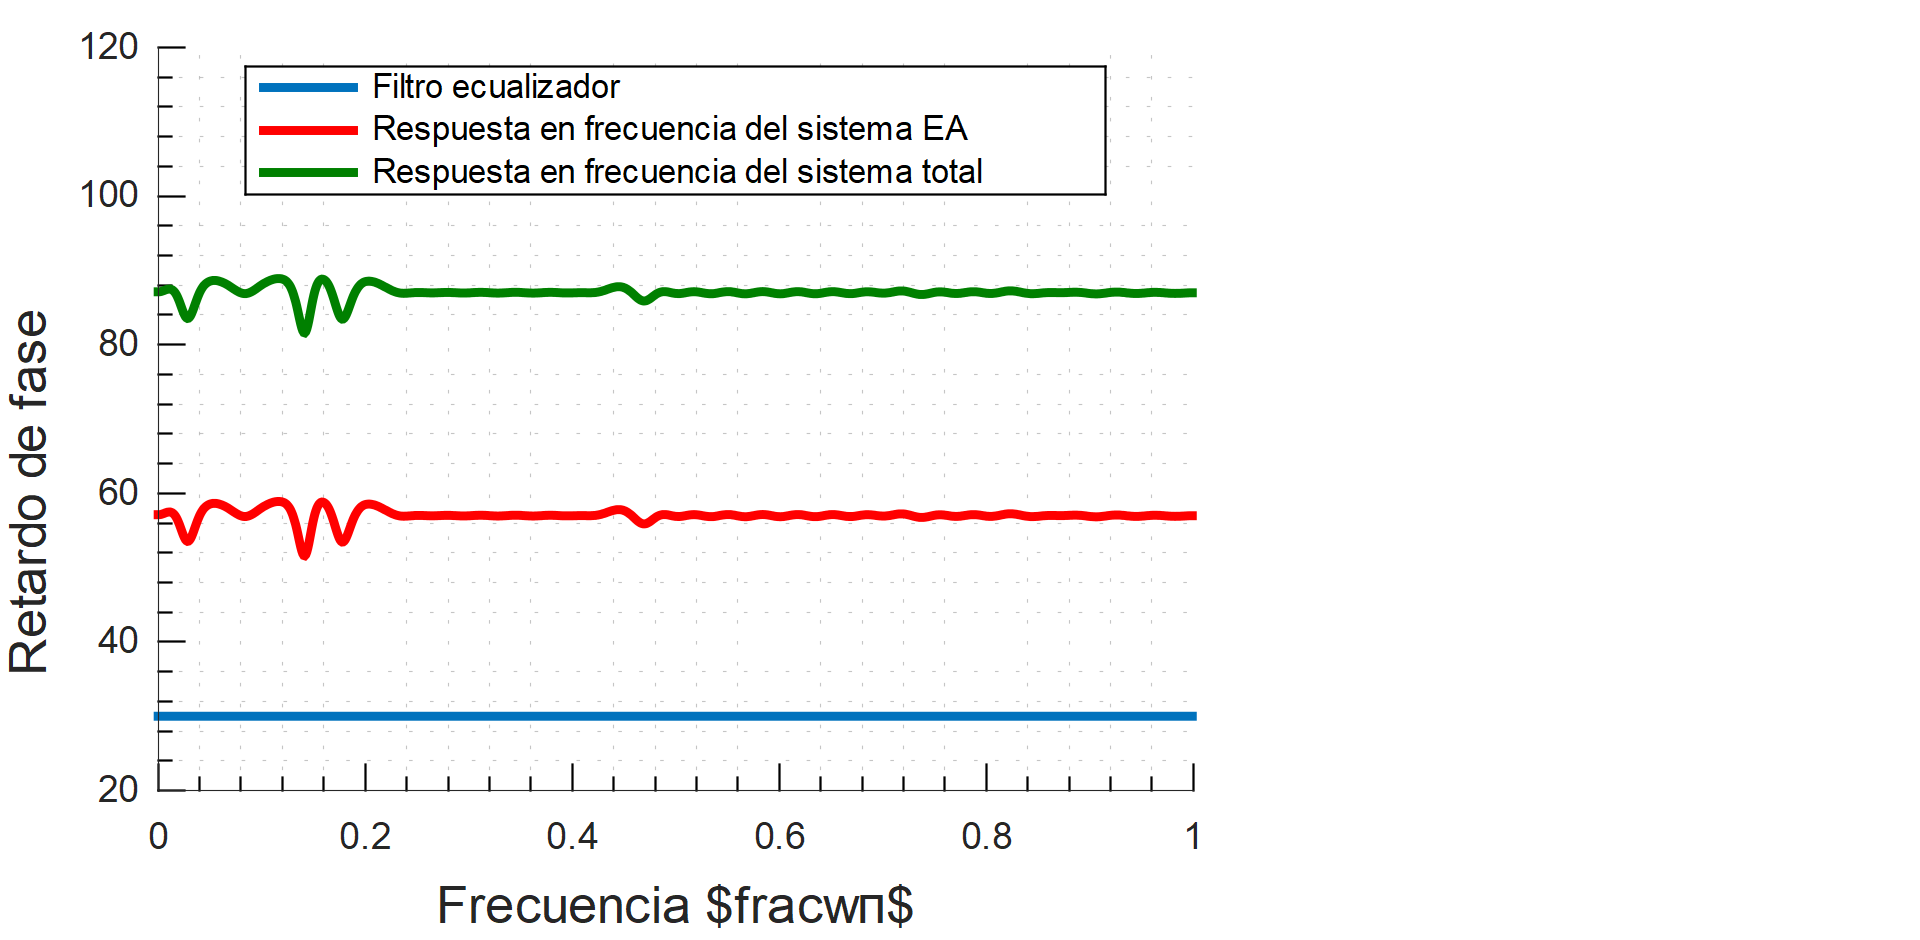
\includegraphics[width=0.9\textwidth]{P12b_retardo_fase.png}
%		\caption{\label{fig:P12b_retardo_fase}Retardo de fase que introduce el filtro ecualizador, el sistema EA y el sistema total.}
%	\end{figure}
	
	Por tratarse del diseño de un filtro de fase lineal, se esperaba aquí también observar un retardo de fase constante. En este método se obtuvo un retardo de 30, un valor menor que con el método de ventanas aplicado (45) a causa de que el orden del filtro es menor. Más allá del valor absoluto del retardo, es de importancia notar que el valor es constante para todas las frecuencias en el rango audible; para aplicaciones de audio, un retardo de fase variable con la frecuencia modifica la forma en que se escucharán las pistas que pasen por el sistema.
	

% Ventajas y desventajas respecto del metodo de 2.1.1



	\section{Parte II: Ecualización mediante filtros de fase no lineal}\label{sec:parteii}
                En esta parte se utilizan técnicas basadas en filtros IIR para el diseño del ecualizador.
{\color{red}{MMM medio figaza ésto pareciera}}

\subsection{Filtro IIR}

%A partir de la respuesta impulsiva del sistema h[n] suministrada, se pide obtener un ecualizador HEQ(ejw) mediante un filtro que compense la respuesta en frecuencia en módulo del sistema EA implementando su sistema inverso, pero al mismo tiempo garantizando las condiciones de estabilidad. Qué tipo de sistemas resultarán de utilidad para este n? Dado que en este caso el filtro se obtiene directamente en función del sistema a compensar, no es necesario definir tolerancias ni especificaciones del mismo.



\subsubsection{Ítem a: transferencia del ecualizador} \label{sec:221a}

	Para que el sistema inverso compensador sea estable, el sistema distorsionador (en nuestro caso, el sistema electroacústico) debe ser estable. Dicha compensación es posible sólo si el sistema EA es de fase mínima.\\

	Suponiendo que el sistema EA tiene función de transferencia racional, se puede descomponer en el producto de una de fase mínima y otra pasa todo. Dado que la respuesta impulsiva es de longitud finita, los polos del sistema se encuentran en el origen o en el infinito. Siendo $n$ la cantidad de ceros del sistema, éste se puede escribir como: 
		
		\begin{equation}
			H_{EA}(z) = \prod^n_{k=1} \frac{1-c_k z^{-1}}{1} 
			\label{eq:prod_hea}
		\end{equation}
	
		El sistema de fase mínima se puede formar a partir de los ceros que se encuentran dentro del círculo unitario y de la reflexión de los que se encuentran fuera a su posición inversa conjugada (siendo ésta en el interior de $|z|<1$). De la ecuación \eqref{eq:prod_hea}, con $m$ ceros tal que $|c_k|>1$, se obtiene:

		\begin{equation*}
			H_{min}(z) = \prod^{n-m-1}_{k=1} \frac{1-c_k z^{-1}}{1} \cdot \prod^{n}_{k=n-m} c_{k} \cdot \frac{1-\overline{c_k^{-1}} z^{-1}}{1}
		\end{equation*}

	Así, con $H_{EA}(z) = H_{min}(z) \cdot H_{ap}(z)$, se define al sistema ecualizador como:

		\begin{equation*}
			H_{IIR}(z)  = \frac{1}{H_{min}(z)}
		\end{equation*}

	De esta forma, el sistema total $H_{total}(z)$ resulta:
		\begin{align*}
			H_{total}(z) &= H_{IIR}(z) \cdot H_{EA}\\
			H_{total}(z) &= H_{ap}(z)\\
			\Rightarrow |H_{total}(z)| &= |H_{ap}(z)| = 1
		\end{align*}


\subsubsection{Ítem b: diagrama de polos y ceros}

	\graficarEPS{0.6}{graf_P21b_HEQ}{Filtro ecualizador.}{fig:P21b_HEQ}
	\graficarEPS{0.6}{graf_P21b_HEA}{Sistema electroacústico.}{fig:P21b_HEA}
	\graficarEPS{0.6}{graf_P21b_HT}{Sistema total.}{fig:P21b_HT}
	
	Como se puede ver en la Figura \ref{fig:P21b_HEQ} el ecualizador tiene todos los polos dentro del círculo unitario, asegurando la estabilidad del filtro. Finalmente, en la Figura \ref{fig:P21b_HT}, se encuentra la misma configuración de ceros del sistema electroacústico (Figura \ref{fig:P21b_HEA}) con la respectiva cancelación dada por el filtro ecualizador. Así la respuesta en módulo del sistema final es constantemente 1.

\subsubsection{Ítem c: respuesta en frecuencia}

	\graficarEPS{0.5}{graf_P21c_rta_frec}{Módulo de la respuesta en frecuencia del filtro, sistema electroacústico y el sistema total.}{fig:21c_rta_frecuencia}

	Del análisis de la Figura \ref{fig:21c_rta_frecuencia} se puede concluir que el filtro diseñado cumple el requerimiento de compensar el sistema original, logrando que la respuesta final del sistema sea plana. Esto se debe a que la respuesta en frecuencia del mismo es exactamente inversa a la del sistema electroacústico. 
	
	Sin embargo, al graficar únicamente el módulo de la transferencia total como se hace en la Figura \ref{fig:P21c_rta_total}, se aprecia un error menor a $\pm \SI{0.003}{\dB}$. Se desconocen las causas del mismo, dado que no se puede atribuir a un error numérico, porque éste debería ser del orden de \num{e-12} o menor. Restaría descartar la implementación de las funciones utilizadas en la pequeña porción de código generado para el cálculo del filtro. 

	\graficarEPS{0.5}{graf_P21c_rta_tot}{Módulo en \si{\dB} de la transferencia total.}{fig:P21c_rta_total}

%	% Se cumple el requerimiento estipulado inicialmente?
%	

\subsubsection{Ítem d: retardo de fase}

	\graficarEPS{0.6}{graf_P21d_retardo_fase}{Retardo de fase que introduce el filtro ecualizador, el sistema EA y el sistema total.}{fig:P21d_retardo_fase}

	A diferencia de los filtros \emph{FIR FLG} y de cuadrados mínimos, el retardo de fase introducido por el filtro es distinto de una constante. Más precisamente, no es lineal. A partir de los cálculos realizados en la Sección \ref{sec:221a} que concluyen que el sistema total se comporta como $H_{ap}(z)$, se determina que la fase del filtro es similar a $H_{ap}(z)$ dado que el retardo del sistema sin compensar no varía más de $\pm 8$ muestras. Sin embargo, el sistema final tiene variaciones de aproximadamente 20 muestras al igual que el filtro.

                
    \section{Audios de prueba y conclusiones}\label{sec:audios}
                	Una vez diseñado y caracterizado cada filtro, se utilizan distintos fragmentos de canciones como posibles señales de prueba que podría entregarle el sistema electroacústico al ecualizador. A través de cinco audios de características y géneros muy diversos, se realizan observaciones sobre la efectividad de cada filtro diseñado para poder reproducirlos como se desearía escucharlos. Las observaciones son tanto subjetivas como objetivas.
	
	\subsection{Audio 1: \emph{Get Lucky - Daft Punk}}
	
%	Cuando pasaa por el EA, el bajo se escucha similar, al igual que la guitarra. Sin embargo, lo que más se ve alterado es la voz principal y los coros. El filtro FLG es el que más se acerca a replicar al original. El que resulta de la utilización del filtro de fase no lineal se encuentra distorsinado por fase fuertemente. Ésta distorsión se ve al escuchar los coros cuando dice \emph{"(...) who we are"}. Las voces de los coros se encuentran más distanciadas de la principal, resultando en un canon más que en un efecto de coro/eco que es el que se escucha en la pista original. En cuanto al diseñado por cuadrados mínimos, se encuentra un leve desplazamiento de dichos coros, pero es imperceptible si no estuviese bajo análisis riguroso.
	La distorsión introducida por el sistema electroacústico se presenta principalmente en las voces y coros, siendo las guitarras y bajos bastante similares a la original. Los filtros de fase lineal replican con bastante fidelidad la porción de audio original y a opinión personal el filtro por ventaneo es mejor. Ésto puede deberse al sobrepico presente en el de cuadrados mínimos, pero es imperceptible la diferencia si se tuviesen las pistas por separado sin saber cómo fueron generadas. Por otro lado, la pista resultante de la utilización del filtro de fase no lineal presenta cambios apreciables. En el estribillo, cuando canta \emph{"(...) who we are"} y aparecen los coros, éstos se encuentran más distanciados de la voz principal que la original. Así, resulta en un efecto de \emph{canon} en vez de un coro o eco que era lo que se oye en la pista original.
	
	
	\subsection{Audio 2: \emph{Música clásica}}
		
	No parece haber mayores diferencias entre la original y las distintas compensaciones.
		
	\subsection{Audio 3: \emph{Beggar's Dance - Jinjer}}
	
%	Extraño. Para el FLG, se escucha un realce de bajos sutil. Con el iir, la voz de la cantante sale del plano central (al haber distorsión de fase, debe perder energía el conjunto de tónicas y armónicas que componen la voz). En este caso, el filtro por cuadrados mínimos me pareció el más acertado. El sistema electroacústico parece sólo a ver afectado el bajo, la pandereta y la voz. Tal vez el redoblante un poco. Lo hace menos medioso (ecualización en V), más nazal.
	En este caso el sistema electroacústico parece afectar sólo al bajo, pandereta (tal vez el redoblante) y voz, sonando más nazal debiendose posiblemente a la disminusión de la banda media de frecuencias. En cuanto a los filtros, el comportamiento es similar al del primer audio. Los de fase lineal se asemejan al original, en particular el de ventaneo tiene un realce de bajos sutil en mi opinión siendo mejor el de cuadrados mínimos, mientras que el de fase no lineal pierde fidelidad. Con el filtro \emph{IIR} pareciera que la voz de la cantante sale del plano central y ésto se puede deber a que la distorsion de fase haga que la tónica y sus armónicas no lleguen al mismo tiempo, perdiendo energía y así su presencia en la mezcla final.
			
	\subsection{Audio 4: \emph{Symphony X - Serpent's Kiss}}
	
	Nuevamente, el sistema parece hacer menos mediosa la mezcla. El filtro \emph{IIR} no ecualiza del todo bien. Le faltan subir medios. El FLG sube un poco de más los medios (se escucha con que las guitarras están un poco más 'adelante'). El original tiene como ggr la guitarra, el flg lo tiene más mrr, iir está apagada la guitarra y el de cuadrados mínimos es más ffr (espero mica que tenga sentido lo que digo). El de cuadrados mínimos queda un poquito corto con los medios.

				
	\subsection{Audio 5: \emph{Game of Thrones Intro}}
	
	De vuelta, el \emph{IIR} lo deja apagado. Ahora vuelve a aparecer el efecto de Get Lucky pero con los violines de la sección intermedia. También resalta al chelo inicial. Después, el FLG y el de cuadrados mínimos no tienen mayores diferencias.

	\subsection{Breve conclusión del análisis empírico de los filtros}

	Las diferencias entre los filtros se suponen deben ser: debido a la ecualización especial del tema (como en la pista 4) o por efectos de post producción como los delays y overdubbs de las canciones más pop. Cuando se encuentran temas con varios instrumentos generando los efectos de forma natural, la distorsión de fase no pareciera ser muy apreciable exceptuando el caso del \emph{IIR} que parece descompensar las frecuencias medias bajandolas levemente, haciendo que todo sea más chato (pero no plano de $|H|=1$ si no de falta de protagonismo).

	
	%\appendix
\end{document}
